\chapter{Work and Energy}

In this chapter, we are going to talk about how engineers define work
and energy. It frequently takes force to get work done. Let's start with thinking 
about the relationship between force and energy. As we learned earlier, Force is 
measured in newtons, and one newton is equal to the force necessary to accelerate 
one kilogram at a rate of $1 m/s^2$.

When you lean on a wall, you are exerting a force on the wall, but you
aren't doing any work. On the other hand, if you push a car for a mile,
you are clearly doing work. Work, to an engineer, is the force you
apply to something, as well as the distance that something moves, in the direction
of the applied force. We measure work in \textit{joules}. A joule is one
newton of force applied over one meter.\index{Joule}

\begin{center}
\includegraphics[width=0.6\textwidth]{workvsforce.png}
\end{center}

For example, if you push a car with a force of 10 newtons for 12
meters, you have done 120 joules of work.\index{work}

\begin{mdframed}[style=important, frametitle={Formula for Work}]
\[
W = F \cdot d
\]

where $W$ is the work in joules, $F$ is the \textit{force} in newtons, and $d$ is 
the distance in meters.

If the force is not in the same direction as the distance, we can use the cosine 
of the angle between the force and the distance:
\[
W = F \cdot d \cdot \cos(\theta)
\]

where $\theta$ is the angle between the force and the distance.
\end{mdframed}

The work-energy theorem (or work-energy principle) states that the net work done 
on an object is equal to the \textbf{change in its kinetic energy}. In other 
words, if you do work on an object, you are changing its kinetic energy. This is 
derived from Newton's second law of motion, covered in the previous chapter. 

% link here to the previous chapter 
%the work-energy theorem only relates to kinetic energy, The extended work-energy principle breaks net work into external and internal (conservative) forces and includes potential energy. I think we should reserve that for a later chapter and stick with the basic concept of delta KE = W = F dot d - Max

\[
W = \Delta E = \Delta KE \text{(with units of Joules (J) or Newton-meters (Nm))} 
\]


Work is how energy is transferred from one thing to another. When you push the 
car, you also burn sugars (energy of the body) in your blood. That energy is then
transferred to the car after it has been pushed uphill.

Thus, we measure the energy something consumes or generates in units of work: 
joules, kilowatt-hours, horsepower-hours, foot-pounds, BTUs (British Thermal 
Unit), and calories.

Let's go over a few different forms that energy can take.

\section{Forms of Energy}\index{energy!Forms of}

In this section we are going to learn about several different types of energy:
\begin{itemize}
\item Heat
\item Electricity
\item Chemical Energy
\item Kinetic Energy
\item Gravitational Potential Energy
\end{itemize}

\subsection{Heat}\index{heat}

When you heat something, you are transferring energy to it. The BTU is a common 
unit for heat. One BTU is the amount of heat required to raise the temperature of 
one pound of water by one degree. One BTU is about 1,055 joules. In fact, when 
you buy and sell natural gas as fuel, it is priced by the BTU.\index{heat} \index{BTU}

\subsection{Electricity}\index{electricity}

Electricity is the movement of electrons. When you push electrons through a space 
that resists their passage (like a light bulb), energy is transferred from the 
power source (like a battery) into the source of the resistance.

Let's say your lightbulb consumes 60 watts of electricity, and you leave it on 
for 24 hours. We would say that you have consumed 1.44 kilowatt hours, or 
3,600,000 joules.


\subsection{Chemical Energy}\index{chemical energy}

As mentioned earlier, some chemical reactions consume energy and some produce 
energy. This means energy can be stored in the structure of a molecule. When a 
plant uses photosynthesis to rearrange water and carbon dioxide into a sugar 
molecule, it converts the energy in the sunlight (solar energy) into chemical 
energy. Remember that photosynthesis is a process that consumes energy. 
Therefore, the sugar molecule has more chemical energy than the carbon dioxide 
and water molecules that were used in its creation.
% ADD: photosythesis equation 
% This was included in one of the previous quizzes, but it is worth repeating here.
% C6H12O6 + 6 O2 -> 6 CO2 + 6 H2O + energy
% KA: https://www.khanacademy.org/science/ap-biology/cellular-energetics/photosynthesis/a/intro-to-photosynthesis

In our diet, we measure this energy in \textit{kilocalories}. A calorie is the 
energy necessary to raise one gram of water one degree Celsius, and is about 
4.19 joules. This is a very small unit. An apple has about 100,000 calories (100 
kilocalories), so people working with food started measuring everything in kilocalories.\index{calories}
% ADD: Conversion chapter should come before this chapter

Here is where things get tricky: People who work with food got tired of saying 
``kilocalories'', so they just started using ``Calorie'' to mean 1,000 calories. 
This has created a great deal of confusion over the years. So if the C is capitalized,
 ``Calorie'' probably means kilocalorie.

\subsection{Kinetic Energy}\index{kinetic energy}

A mass in motion has energy. For example, if you are in a moving car and you slam 
on the breaks, the energy from the motion of the car will be converted into heat 
in the breaks and under the tires.

How much energy does the car have?
\[
E = \frac{1}{2} m v^2
\]

\begin{mdframed}[style=important, frametitle={Formula for Kinetic Energy}]

\[
E = \frac{1}{2} m v^2
\]

where $E$ is the energy in joules, $m$ is the mass in kilograms, and
$v$ is the speed in meters per second.

\end{mdframed}

\subsection{Gravitational Potential Energy}\index{potential energy!gravitational}


When you lift something heavy onto a shelf, you are giving it \textit{potential 
energy}. The amount of energy that you transferred to it is proportional to its 
weight and the height that you lifted it.

\[
E = mgh
\]
a rate of $9.8 m/s^2$.

\begin{mdframed}[style=important, frametitle={Formula for Gravitational Potential Energy}]
The formula for gravitational potentional energy is

\[
E = mgh
\]

where $E$ is the energy in joules, $m$ is the mass of the object you
lifted, $g$ is acceleration due to gravity, and $h$ is the height that you lifted it.

On earth, then, gravitational potential energy is given by

\[
E = (9.8)mh
\]

since objects in free-fall near Earth's surface accelerate at $9.8 m/s^2$.

\end{mdframed}


There are other kinds of potential energy. For example, when you draw a bow in 
order to fire an arrow, you have given that bow potential energy. When you release it,
the potential energy is transferred to the arrow, which expresses it as kinetic energy.
% ADD: section about KE and U

\section{Conservation of Energy}

The first law of thermodynamics says ``Energy is neither created nor destroyed.''
\index{energy!conservation of}

Energy can change forms. Your cells consume chemical energy to give gravitational 
potential energy to a car you push up a hill. However, the total amount of energy 
in a closed system stays constant. 
%in the conservation of energy chapter, we discussed open, closed, and isolated systems. technically, the energy in an isolated system stays constant, while the change in energy of a closed system is equal to the flow of energy across the system boundary. Should we change this to "isolated" or explain how energy is accounted for in a closed system? -Max

\begin{Exercise}[title={The Energy of Falling}, label=energy_falling]

A 5 kg cannonball falls off the top of a 3 meter ladder. As it falls, its 
gravitational potential energy is converted into kinetic energy. How fast is 
the cannonball traveling just before it hits the floor?

\end{Exercise}
\begin{Answer}[ref=energy_falling]

  At the top of the ladder, the cannonball has $(9.8)(5)(3) = 147$ joules of potential energy.

  At the bottom, the kinetic energy $\frac{1}{2}(5)v^2$ must be equal
  to 147 joules. So $v^2 = \frac{294}{5}$.  This means it is going about
  $7.7$ meters per second.

  (You may be wondering about air resistance. Yes, a tiny amount of energy is 
  lost to air resistance, but for a dense object moving at these relatively slow 
  speeds, this energy is negligible.)

\end{Answer}

\section{Work and Kinetic Energy}
As stated above, the work-energy theorem tells us that the change in an object's 
kinetic energy is equal to the work done on that object. For now, we will only 
consider examples where the force and the direction of motion are parallel or 
perpendicular. When you learn about vectors, we will expand this to include 
forces that are skew to the direction of motion. 

Consider what happens when you toss a ball in the air: once the ball leaves your 
hand, the only force acting on it is gravity. Initially, the ball is moving 
upwards while gravity points downwards:

\begin{center}
    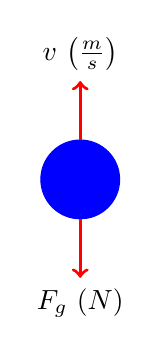
\begin{tikzpicture}
        \draw[blue, fill=blue] (0,0) circle (0.5cm);
        \draw[->, very thick, red] (0, 0.5) -- (0, 1.25) node[above, black] 
        {$v$ $\left( \frac{m}{s} \right)$};
        \draw[->, very thick, red] (0, -0.5) -- (0, -1.25) node[below, black] 
        {$F_g$ $\left( N \right)$};
    \end{tikzpicture}
\end{center}

Intuitively, we know that the ball will slow down (lose kinetic energy) as it 
moves upwards:

$$\Delta KE < 0$$

Since $W = \Delta KE$, we also know that gravity must be doing \textit{negative 
work}. Whenever the direction of the force is opposite the direction of the 
motion, the work done by that force is negative. 

\textbf{Example}: if the ball has a mass of 0.5 kg, how much kinetic energy 
does it lose as it moves upwards by 1 m?

\textbf{Solution}: The force acting on the ball is its weight, $F_w = mg$, and we 
will designate this as negative since weight points downwards. Using the 
work-energy theorem, 

$$\Delta KE = F \cdot d = \left( mg \right) \cdot d = \left( 0.5 kg \right) \left(
-9.8 \frac{m}{s^2} \right) \left( 1 m \right) = -4.9 J$$

Therefore, the ball loses 4.9 joules of kinetic energy for every 1 meter it moves 
upwards (the fact it is \textit{losing kinetic energy} is represented by the 
result being negative).

\begin{Exercise}[title = {How far will you slide?}, label = slide]
You are playing softball and have to slide into home. If you sprint at a maximum 
of 10 m/s and the force of friction between you and the ground is 0.3 times your 
weight, how far from the base can you start your slide and still reach home?
\end{Exercise}

\begin{Answer}[ref = slide]
$$F_f \cdot d = \Delta KE = KE_f - KE_i$$

You'll reach the maximum distance you can slide when you stop moving, so we will 
use a final velocity of zero, which means a final kinetic energy of zero:
$$F_f \cdot d = -KE_i = \frac{1}{2}mv^2$$

Since the force of friction is 0.3 times your weight, we know that:
$$F_f = 0.3 F_w = 0.3mg$$

Substituting and canceling the mass:
$$\left( 0.3 mg \right) \cdot d = \frac{1}{2}mv^2$$
$$0.3g \cdot d = \frac{1}{2}v^2$$

Since we know g and v, we can solve for d:
$$d = \frac{v^2}{0.6g} = \frac{\left( 10 \frac{m}{s} \right)^2}{0.6 \left( 9.8 
\frac{m}{s^2} \right)} \approx 1.7 m$$

So, if you want to reach home base, you should start your slide no more than 
1.7 m from home. 
\end{Answer}

\begin{Exercise}[title = {Ranking Stopping Force}, label = stop]
In drag racing, cars can reach speeds of 150 miles per hour (approximately 240 
kilometers per hour). In order to be able to stop quickly and safely, drag 
racing cars are built with parachutes that deploy at the end of the race. 
Consider a drag race where cars of different masses reach different maximum 
speeds. There is 100 meters between the finish line and the fence surrounding 
the race track. If all the race cars deploy their parachutes at the finish line 
while going their maximum speed, rank the force needed from the parachute to 
stop each car in the required distance from least to greatest:

\begin{center}
	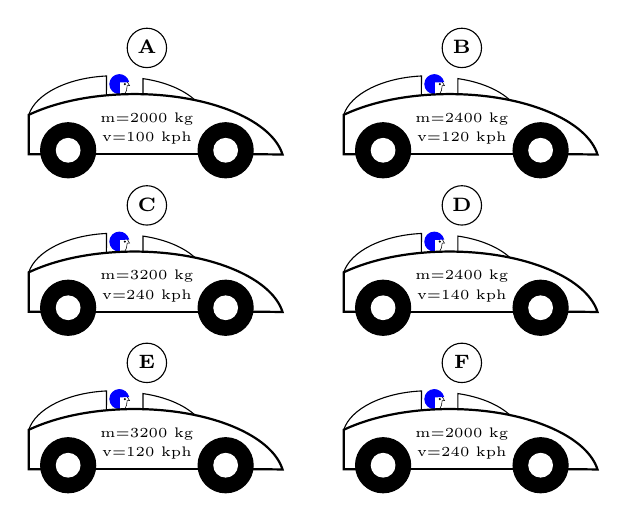
\begin{tikzpicture}
            %CAR A
            %tires
            \draw[black, fill=black] (0.5, 4.35) circle (0.35);
            \draw[white, fill=white] (0.5, 4.35) circle (0.15);
            \draw[black, fill=black] (2.5, 4.35) circle (0.35);
            \draw[white, fill=white] (2.5, 4.35) circle (0.15);

            %driver
            \draw[very thin] (1.25, 5.22) -- (1.28, 5.17) -- (1.25, 5.17) 
            	arc (0:-35:0.2cm and 0.2cm);
            \draw[blue, fill=blue] (1.15, 5.07) arc (270:15:0.12) -- (1.15, 5.22) -- cycle;
            \draw[black, fill=black] (1.22, 5.19) circle (0.05mm);
            
            %outline
            \draw[black, thick] (0.8, 4.3) -- (2.2, 4.3);
            \draw[black, thick] (0.2, 4.3) -- (0, 4.3) -- (0, 4.8) 
            	arc (135:8.5:1.9cm and 0.9cm) -- (2.8, 4.3);
            \draw[black] (0, 4.8) arc (170:95:1.1cm and 0.6cm) -- (.986, 5.05); 
            \draw[black] (1.45, 5.05) -- (1.45, 5.26) arc (75:30:1.1cm and 0.6cm); 

            %speed and mass info
            \node[font=\tiny] at (1.5, 4.75) {m=2000 kg};
            \node[font=\tiny] at (1.5, 4.5) {v=100 kph};

            %car label
            \draw[black] (1.5, 5.65) circle (0.25) 
            	node[above, font = \scriptsize, yshift = -0.2cm] {\textbf{A}};

            %CAR B
            %tires
            \draw[black, fill=black] (4.5, 4.35) circle (0.35);
            \draw[white, fill=white] (4.5, 4.35) circle (0.15);
            \draw[black, fill=black] (6.5, 4.35) circle (0.35);
            \draw[white, fill=white] (6.5, 4.35) circle (0.15);

            %driver
            \draw[very thin] (5.25, 5.22) -- (5.28, 5.17) -- (5.25, 5.17) 
            	arc (0:-35:0.2cm and 0.2cm);
            \draw[blue, fill=blue] (5.15, 5.07) arc (270:15:0.12) -- (5.15, 5.22) -- cycle;
            \draw[black, fill=black] (5.22, 5.19) circle (0.05mm);
            
            %outline
            \draw[black, thick] (4.8, 4.3) -- (6.2, 4.3);
            \draw[black, thick] (4.2, 4.3) -- (4, 4.3) -- (4, 4.8) 
            	arc (135:8.5:1.9cm and 0.9cm) -- (6.8, 4.3);
            \draw[black] (4, 4.8) arc (170:95:1.1cm and 0.6cm) -- (4.986, 5.05); 
            \draw[black] (5.45, 5.05) -- (5.45, 5.26) arc (75:30:1.1cm and 0.6cm); 

            %speed and mass info
            \node[font=\tiny] at (5.5, 4.75) {m=2400 kg};
            \node[font=\tiny] at (5.5, 4.5) {v=120 kph};

            %car label
            \draw[black] (5.5, 5.65) circle (0.25) 
            	node[above, font = \scriptsize, yshift = -0.2cm] {\textbf{B}};
            
            %CAR C
            %tires
            \draw[black, fill=black] (0.5, 2.35) circle (0.35);
            \draw[white, fill=white] (0.5, 2.35) circle (0.15);
            \draw[black, fill=black] (2.5, 2.35) circle (0.35);
            \draw[white, fill=white] (2.5, 2.35) circle (0.15);

            %driver
            \draw[very thin] (1.25, 3.22) -- (1.28, 3.17) -- (1.25, 3.17) 
            	arc (0:-35:0.2cm and 0.2cm);
            \draw[blue, fill=blue] (1.15, 3.07) arc (270:15:0.12) -- (1.15, 3.22) -- cycle;
            \draw[black, fill=black] (1.22, 3.19) circle (0.05mm);
            
            %outline
            \draw[black, thick] (0.8, 2.3) -- (2.2, 2.3);
            \draw[black, thick] (0.2, 2.3) -- (0, 2.3) -- (0, 2.8) 
            	arc (135:8.5:1.9cm and 0.9cm) -- (2.8, 2.3);
            \draw[black] (0, 2.8) arc (170:95:1.1cm and 0.6cm) -- (.986, 3.05); 
            \draw[black] (1.45, 3.05) -- (1.45, 3.26) arc (75:30:1.1cm and 0.6cm); 

            %speed and mass info
            \node[font=\tiny] at (1.5, 2.75) {m=3200 kg};
            \node[font=\tiny] at (1.5, 2.5) {v=240 kph};

            %car label
            \draw[black] (1.5, 3.65) circle (0.25) 
            	node[above, font = \scriptsize, yshift = -0.2cm] {\textbf{C}};

            %CAR D
            %tires
            \draw[black, fill=black] (4.5, 2.35) circle (0.35);
            \draw[white, fill=white] (4.5, 2.35) circle (0.15);
            \draw[black, fill=black] (6.5, 2.35) circle (0.35);
            \draw[white, fill=white] (6.5, 2.35) circle (0.15);

            %driver
            \draw[very thin] (5.25, 3.22) -- (5.28, 3.17) -- (5.25, 3.17) 
            	arc (0:-35:0.2cm and 0.2cm);
            \draw[blue, fill=blue] (5.15, 3.07) arc (270:15:0.12) -- (5.15, 3.22) -- cycle;
            \draw[black, fill=black] (5.22, 3.19) circle (0.05mm);
            
            %outline
            \draw[black, thick] (4.8, 2.3) -- (6.2, 2.3);
            \draw[black, thick] (4.2, 2.3) -- (4, 2.3) -- (4, 2.8) 
            	arc (135:8.5:1.9cm and 0.9cm) -- (6.8, 2.3);
            \draw[black] (4, 2.8) arc (170:95:1.1cm and 0.6cm) -- (4.986, 3.05); 
            \draw[black] (5.45, 3.05) -- (5.45, 3.26) arc (75:30:1.1cm and 0.6cm); 

            %speed and mass info
            \node[font=\tiny] at (5.5, 2.75) {m=2400 kg};
            \node[font=\tiny] at (5.5, 2.5) {v=140 kph};

            %car label
            \draw[black] (5.5, 3.65) circle (0.25) 
            	node[above, font = \scriptsize, yshift = -0.2cm] {\textbf{D}};
            
            %CAR E
            %tires
            \draw[black, fill=black] (0.5, 0.35) circle (0.35);
            \draw[white, fill=white] (0.5, 0.35) circle (0.15);
            \draw[black, fill=black] (2.5, 0.35) circle (0.35);
            \draw[white, fill=white] (2.5, 0.35) circle (0.15);

            %driver
            \draw[very thin] (1.25, 1.22) -- (1.28, 1.17) -- (1.25, 1.17) 
            	arc (0:-35:0.2cm and 0.2cm);
            \draw[blue, fill=blue] (1.15, 1.07) arc (270:15:0.12) -- (1.15, 1.22) -- cycle;
            \draw[black, fill=black] (1.22, 1.19) circle (0.05mm);
            
            %outline
            \draw[black, thick] (0.8, 0.3) -- (2.2, 0.3);
            \draw[black, thick] (0.2, 0.3) -- (0, 0.3) -- (0, 0.8) 
            	arc (135:8.5:1.9cm and 0.9cm) -- (2.8, 0.3);
            \draw[black] (0, 0.8) arc (170:95:1.1cm and 0.6cm) -- (.986, 1.05); 
            \draw[black] (1.45, 1.05) -- (1.45, 1.26) arc (75:30:1.1cm and 0.6cm); 

            %speed and mass info
            \node[font=\tiny] at (1.5, 0.75) {m=3200 kg};
            \node[font=\tiny] at (1.5, 0.5) {v=120 kph};

            %car label
            \draw[black] (1.5, 1.65) circle (0.25) 
            	node[above, font = \scriptsize, yshift = -0.2cm] {\textbf{E}};

            %CAR F
            %tires
            \draw[black, fill=black] (4.5, 0.35) circle (0.35);
            \draw[white, fill=white] (4.5, 0.35) circle (0.15);
            \draw[black, fill=black] (6.5, 0.35) circle (0.35);
            \draw[white, fill=white] (6.5, 0.35) circle (0.15);

            %driver
            \draw[very thin] (5.25, 1.22) -- (5.28, 1.17) -- (5.25, 1.17) 
            	arc (0:-35:0.2cm and 0.2cm);
            \draw[blue, fill=blue] (5.15, 1.07) arc (270:15:0.12) -- (5.15, 1.22) -- cycle;
            \draw[black, fill=black] (5.22, 1.19) circle (0.05mm);
            
            %outline
            \draw[black, thick] (4.8, 0.3) -- (6.2, 0.3);
            \draw[black, thick] (4.2, 0.3) -- (4, 0.3) -- (4, 0.8) 
            	arc (135:8.5:1.9cm and 0.9cm) -- (6.8, 0.3);
            \draw[black] (4, 0.8) arc (170:95:1.1cm and 0.6cm) -- (4.986, 1.05); 
            \draw[black] (5.45, 1.05) -- (5.45, 1.26) arc (75:30:1.1cm and 0.6cm); 

            %speed and mass info
            \node[font=\tiny] at (5.5, 0.75) {m=2000 kg};
            \node[font=\tiny] at (5.5, 0.5) {v=240 kph};

            %car label
            \draw[black] (5.5, 1.65) circle (0.25) 
            	node[above, font = \scriptsize, yshift = -0.2cm] {\textbf{F}};
	\end{tikzpicture}
\end{center}
\end{Exercise}

\begin{Answer}[ref = stop]
Since all the cars need to stop in the same distance, the cars with the 
greatest kinetic energy will take the most force to stop. Calculating the 
kinetic energies (we won't change the units from kilometers per hour to meters 
per second, since we're just comparing the values):

\begin{center}
	\begin{tabular}{|c|c|c|c|}\hline
	Car & Mass [kg] & Max speed [kph] & KE [kg $(kph)^2$]\\\hline
	A & 2000 & 100 & $1 \times 10^7$\\\hline
	B & 2400 & 120 & $1.728 \times 10^7$\\\hline
	C & 3200 & 240 & $9.216 \times 10^7$\\\hline
	D & 2400 & 140 & $2.352 \times 10^7$\\\hline
	E & 3200 & 120 & $2.304 \times 10^7$\\\hline
	F & 2000 & 240 & $5.67 \times 10^7$\\\hline
	\end{tabular}
\end{center}

The correct ranking is A, B, E, D, F, C. 
\end{Answer}

\subsection{Forces that do no work}
If the object you are pushing doesn't move. or the applied force is perpendicular 
to the direction of motion, that force does no work. Let's look at a few examples:

\subsubsection{Pushing Against an Immobile Object}
At the beginning of the chapter, we said that when you push on a wall, you don't 
do any work. Why is this? Well, if the wall is a good wall (that is, strong 
enough to not be pushed over by a person), the wall won't move while you push on 
it. This means the distance over which your push is applied is zero, and 
therefore the work done ($F \cdot d = F \cdot 0 = 0$) is zero joules.

\subsubsection{Walking Across a Room with a Book}
Imagine holding a book flat on your hands and walking at a constant velocity. 
Your hand is applying an upwards force to the book, but the book is moving 
horizontally. This means the force and direction of motion are 
\textit{perpendicular}. Recall from the beginning of the chapter than if the 
force and distance are not parallel, then the work is given by $W = F \cdot d 
\cos{\left( \theta \right)}$. (When the vectors are parallel, $\theta = 0$ and 
$\cos{\left( \theta \right)} = 1$, while when the vectors point in opposite 
directions, $\theta = 180^{\circ}$ and $\cos{ \left( \theta \right)} = -1$.) 
When the vectors are perpendicular, then $\theta = 90^{\circ}$ and $\cos{ \left( 
\theta \right)} = 0$. Therefore, $W = 0$ as well and the upward force of your 
hands does no net work. 

\subsubsection{Circular Motion}
We will discuss circular motion further in a subsequent chapter. For now, know 
that constant-speed circular motion is caused by a constant-magnitude force that 
always points to the center of the circle the object is moving in. For example, 
you can take a weight on the end of a string and spin it. The tension in the 
string spins the weight, and the string always points from the object to your 
hand (the center of the weight's circular path). For a satellite, that force is 
gravitational attraction to the Earth.

\begin{center}
\includegraphics[width=4in]{satellite.png}
\end{center}

As a result, the force changes the \textit{direction}, but not the 
\textit{magnitude} of the satellite's velocity. Let's re-examine the equation 
for kinetic energy:

$$KE = \frac{1}{2}mv^2$$

Since the velocity is squared, the direction of motion doesn't affect the kinetic 
energy (a ball moving at 5 m/s upwards has the same kinetic energy as if the ball 
were moving at 5 m/s downwards). So, a force that causes circular motion doesn't 
change a circling object's kinetic energy, and therefore does no work (as 
expected when force and direction of motion are perpendicular)!

\section{Efficiency}
% Depending on how important this is, we may want to expand this section or give it its own chapter. - Arjan
Although energy is always conserved as it moves through different forms, 
scientists aren't always that good at controlling it.\index{efficiency}

In terms of an equation, efficiency is the ratio of the useful energy output to 
the total energy input. It is usually expressed as a percentage.
\begin{mdframed}[style=important, frametitle={Formula for Efficiency}]
\[
\text{Efficiency} = \frac{\text{Useful Energy Output}}{\text{Total Energy Input}} 
\times 100\%
\]
\end{mdframed}
where the useful energy output is the energy that is actually used to do work or 
complete a task, and the total energy input is the total energy consumed by the 
system.

A machine is considered 100\% efficient only if all the input work is converted 
into useful output work, with no energy lost to heat, friction, or sound. 100\% 
efficient process don't exist in real-life: every process loses some useful 
energy to heat. 

For example, when a car engine consumes the chemical energy in gasoline, only
about 20\% of the energy consumed is used to turn the wheels. Most of the energy 
is actually lost as heat. If you run a car for a while, the engine gets very hot, 
as does the exhaust coming from the tailpipe.

A human is about 25\% efficient. Most of the loss is in the heat produced during 
the chemical reactions that turns food into motion.
% ADD: Cellular Respiration

In general, if you are trying to increase efficiency in any system, the solution 
is usually easy to identify by the heat that is produced. Reduce the heat, increase 
the efficiency.

Light bulbs are an interesting case. To get the same amount of light of a 60 watt 
incandescent bulb, you can use an 8 watt LED or a 16 watt fluorescent light. This 
is why we say that the LED light is much more efficient. If you run both, the 
incandescent bulb will consume 1.44 kilowatt-hours; the LED will consume only 
0.192 kilowatt-hours. 

In addition to light, the incandescent bulb is producing a lot of heat. If it
is inside your house, what happens to the heat? It warms your house.

In the winter, when you want light and heat, the incandescent bulb is
100\% efficient!

Of course, this also means the reverse is true. In the summer, if you are running 
the air conditioner to cool down your house, the incandescent bulb is worse than 
just ``inefficient at making light'' --- it is actually counteracting the air 
conditioner!
